\documentclass[11pt]{article}

\usepackage[margin=0.84in]{geometry}
\usepackage{amsmath}
\usepackage{amssymb}
\usepackage{booktabs}
\usepackage{graphicx}
\usepackage{microtype}
\usepackage{array}
\usepackage{url}
\usepackage{xcolor}
\usepackage[hidelinks]{hyperref}

\definecolor{passgreen}{HTML}{047857}
\definecolor{failred}{HTML}{B91C1C}
\definecolor{resultblue}{HTML}{1D4ED8}
\newcommand{\pass}{\textcolor{passgreen}{\textbf{PASS}}}
\newcommand{\fail}{\textcolor{failred}{\textbf{FAIL}}}
\newcommand{\code}[1]{\texttt{#1}}

\title{\textbf{Hardening a Deterministic ``Neuron'' Interface}\\
\large Frozen Three-Seed Semantic-Curriculum Tests in TinyLlama}
\author{Josiah Wilson\\Independent Researcher}
\date{July 27, 2026}

\begin{document}
\maketitle

\begin{abstract}
We test whether hard semantic-contrast training can repair the learned linear
interface to an existing deterministic addition subspace in frozen
TinyLlama-1.1B. The calculator, its layer-15 placement, 28 assigned SwiGLU
coordinates, 24,576 learned result weights, all pretrained weights, and runtime
state remain fixed. Phase 9 updates only 32,768 route, role, and digit input
weights. Generic and hard continuation use paired source checkpoints,
identical 2,400-example budgets, optimizer schedules, development thresholds,
and three seeds; only their curricula differ.

The exact prompt manifest, 100 additions, 200 adversarial negatives, gates,
and hashes were frozen before confirmatory training or evaluation. Hard
continuation reached 61/100, 61/100, and 58/100 exact additions, versus
59/100, 63/100, and 58/100 for generic continuation and 67/100, 68/100, and
68/100 for the unchanged Phase 8 implant. Hard training increased exact
operand registers to 81--85/100 and reduced Phase 8 false routes from
26--30/200 to 11--12/200. It nevertheless routed off exactly 24/100 additions
per seed and produced more false routes than generic continuation's 8/200.

Every active-route, exact-operand hard execution had an exact deterministic
trajectory and exact decoded answer (61/61, 60/60, and 57/57). Result-channel
ablation reduced all seeds to 0/100 exact. A disclosed evaluator bookkeeping
bug marked this conditional gate false by comparing mismatched aggregate
counts; row-level protocol recomputation makes it the only passing technical
gate. The compound protocol failed because the other five gates failed.

Phase 9 therefore supplies a negative capacity result: semantic contrasts
moved TinyLlama's frozen linear decision boundary and improved specific state
typing, but did not create a robust neural interface. The deterministic
calculator remained exact; routing, typed activation, and operand
representation remain the bottleneck.
\end{abstract}

\section*{Technical summary}

\begin{center}
\small
\begin{tabular}{p{0.48\linewidth}rrr}
\toprule
Confirmatory metric & Seed 15,201 & Seed 15,202 & Seed 15,203\\
\midrule
Hard exact additions & 61/100 & 61/100 & 58/100\\
Hard direct additions & 21/50 & 22/50 & 21/50\\
Hard word problems & 20/25 & 20/25 & 20/25\\
Hard distractor additions & 20/25 & 19/25 & 17/25\\
Hard exact operands & 85/100 & 84/100 & 81/100\\
Hard positive routes / active routes
  & 76 / 72 & 76 / 71 & 76 / 69\\
Conditional exact trajectory and decode
  & 61/61 & 60/60 & 57/57\\
Exact after result ablation & 0/100 & 0/100 & 0/100\\
Hard false routes / preserved negatives
  & 12 / 188 & 12 / 188 & 11 / 189\\
Generic exact additions / false routes
  & 59 / 8 & 63 / 8 & 58 / 8\\
Frozen Phase 8 exact / false routes
  & 67 / 30 & 68 / 26 & 68 / 27\\
Matched-adapter exact additions
  & 21/100 & 14/100 & 20/100\\
\bottomrule
\end{tabular}
\end{center}

\noindent\textbf{Frozen compound verdict:} \fail.

\medskip
\noindent\textbf{Protocol-defined gate verdict:} one of six technical gates
passed. The conditional calculator-and-decode gate passed after row-level
recomputation; accuracy, operands, routing/preservation, causal-count, and
hard-over-generic gates failed.

\medskip
\noindent\textbf{Mechanistic verdict:} support retained. All protocol-defined
valid hard executions were exact, and ablating only the deterministic result
coordinates removed every correct hard answer.

\medskip
\noindent\textbf{Interface verdict:} failure. Hard contrasts improved specific
operand and negative families but reduced addition-route recall and did not
outperform generic continuation.

\section{Motivation and scope}

Flexible neural sequence models and exact algorithms have complementary
strengths. Neural arithmetic architectures and algorithmic-reasoning systems
ask whether explicit structure can improve systematic computation
\cite{trask2018,lindner2023,bounsi2024}. Dietz and Klakow's Integrated Gated
Calculator established direct prior art for a learned calculator module inside
a frozen Llama model \cite{dietz2025}; this work does not claim the broad
integrated-calculator idea as novel.

The narrower hypothesis proposed by Josiah Wilson is that deterministic
programs can occupy neuron-shaped activation slots inside an otherwise
ordinary network. Surrounding neural computation learns when and how to encode
state into those slots and how to use their exact outputs. This is part of a
broader \emph{semi-deterministic AI} program: retain neural interpretation and
flexible representation while embedding compact, auditable deterministic
mechanisms into native activation pathways.

Phase 8 moved a 28-coordinate, zero-learned-parameter addition circuit from
Qwen2.5-0.5B to frozen TinyLlama-1.1B. All correctly typed executions were
arithmetically and causally exact, but a frozen audit failed: each seed
answered only 53/60 additions exactly and falsely routed 9--12/60 adversarial
negatives. Failures clustered in unseen semantic families. The calculator
transferred; its linear natural-language interface did not generalize robustly.

Phase 9 asks one deliberately narrower question: can hard semantic-contrast
training repair that existing interface without moving or modifying the
calculator? It does not test repeated calculator invocation, residual-native
persistent state, multiple operations, a nonlinear readout, surrounding-layer
adaptation, or a more capable base model.

\section{Frozen model and architecture}

\subsection{TinyLlama and in-place activation subspace}

Experiments use
\code{TinyLlama/TinyLlama-1.1B-Chat-v1.0} \cite{tinyllama2024}, revision
\begin{sloppypar}
\code{fe8a4ea1ffedaf415f4da2f062534de366a451e6}.
\end{sloppypar}
The loaded model contains 1,100,048,384 parameters, 22 decoder layers, hidden
width 2,048, and SwiGLU MLP width 5,632. Every pretrained parameter remains
frozen and generation is greedy.

The Phase 8 implant remains at decoder MLP layer 15. Twenty-eight existing
intermediate coordinates are assigned a typed activation ABI:

\begin{center}
\small
\begin{tabular}{lrr}
\toprule
Group & Coordinates & Learned weights\\
\midrule
Route: off/add & 2 & $2\times2{,}048=4{,}096$\\
Token role: none/A/B & 3 & $3\times2{,}048=6{,}144$\\
Digit: 0--9/non-digit & 11 & $11\times2{,}048=22{,}528$\\
Result: 0--9/end/pad & 12 & $12\times2{,}048=24{,}576$\\
\midrule
Total & 28 & 57,344\\
\bottomrule
\end{tabular}
\end{center}

The first 16 rows linearly classify route, operand role, and digit from native
layer-15 states. A typed role/digit handshake supplies up to two four-digit
decimal operands to a frozen ripple-carry adder with zero learned parameters.
One-hot result symbols pass through 12 learned residual columns, then through
TinyLlama's unchanged downstream blocks, final normalization, and language
head.

When the route is off, the selected coordinates' original MLP contribution is
restored exactly. The route is latched on the first response step; the first
valid operands enter a response-local deterministic register; and a
deterministic counter selects successive result digits. These tensors are
disclosed runtime microcircuit state, not learned parameters or
residual-native recurrent state.

\subsection{What Phase 9 changes}

Each Phase 9 run inherits one independent Phase 8 implant checkpoint. It
updates only the 32,768 input-interface weights. The 24,576 learned result
columns must remain bit-identical to the source checkpoint. The calculator,
layer, selected coordinates, result strength, runtime state, base model, and
architectural learned-parameter count remain fixed.

Thus the architecture still contains 57,344 learned weights, or
0.005213\% of TinyLlama. Phase 9 modifies 32,768 weights, or 0.002979\% of the
base. Its deterministic calculator contains no learned weights. Development
calibration changes the digit-confidence threshold from 0.9 to 0.8 without
adding computation or parameters.

\section{Frozen protocol}

\subsection{Conditions and seeds}

All conditions receive the same 300 prompts in the same order:

\begin{enumerate}
\item untouched TinyLlama;
\item the existing rank-14 residual adapter with exactly 57,344 learned
      weights;
\item the unchanged Phase 8 implant;
\item generic Phase 9 continuation;
\item hard-contrast Phase 9 continuation;
\item hard-contrast result-channel ablation on positive prompts.
\end{enumerate}

Phase 9 seeds 15,201, 15,202, and 15,203 inherit Phase 8 seeds 14,201, 14,202,
and 14,203 respectively. Generic and hard continuation use identical source
checkpoints, example counts, trainable weights, optimizer schedules,
development data, and threshold-selection rules. Only the curriculum differs.

\subsection{Curricula and development}

Each continuation set contains 1,200 route-positive additions and 1,200
route-negative prompts. Generic continuation draws from the previous
training-family distribution. Hard continuation balances new semantic
families covering direct addition, reversed surface order, state increments,
unfamiliar operational and scientific word problems, irrelevant identifiers,
operand-final constructions, multiplication, factual numbers, quotation,
negation, cancellation, subtraction, comparison, concatenation, division,
averaging, and hypothetical discussion.

The shared development set contains 240 positives and 480 negatives across 36
families disjoint from both training and confirmation. The initial hard
curriculum improved a balanced generation subset from generic continuation's
32/60 exact additions to 47/60, but missed two operand-final positive
families. Replacing four training families while holding the count fixed
raised the hard condition to 54/60 at threshold 0.9 and an inferred 55/60
after development-only threshold calibration to 0.8. Increasing role/digit
loss weights and extending optimization did not improve end-to-end exactness
and were rejected.

The frozen schedule uses 1,500 interface updates (batch 256, learning rate
0.0005) and 2,500 route-row hardening updates (batch 256, learning rate
0.0005). Route, role, and digit losses have unit weight; learned step loss has
weight zero. The route threshold maximizes development recall subject to a
1\% false-positive cap.

\subsection{Sealed confirmation}

The exact confirmation contains 300 unique prompts:

\begin{itemize}
\item 50 direct additions;
\item 25 word problems;
\item 25 additions with an irrelevant third number;
\item 200 adversarial negatives, 20 each across multiplication, factual
      numbers, quoted arithmetic, negated addition, canceled addition,
      subtraction, comparison, concatenation, hypothetical arithmetic, and
      three-number distractors.
\end{itemize}

All 70 confirmation families use strings not seen in training or development.
Operand pairs are disjoint across Phase 8, Phase 9
training, development, and confirmation. The canonical prompt-row SHA-256
begins \code{ed15e17692c0}; its full value is retained in the tracked
manifest. Greedy decoding uses at most eight generated tokens for every
condition.

The implementation and all retained development outcomes were committed at
\code{52f7e71}. The prompt manifest was committed separately at
\code{6f50db9} before confirmatory training or model evaluation.

\subsection{Metrics and frozen gates}

For every hard-condition seed, the audit records strict numeral-only exact
accuracy, exact operand-register recovery, route prediction and activation,
deterministic calculator trajectories, conditional downstream decoding,
paired result ablation, adversarial false routes, token-exact preservation
relative to untouched base, category failures, local latency, and sampled MPS
memory.

The hard condition passes only if every seed satisfies all six gates:

\begin{enumerate}
\item at least 95/100 exact additions;
\item at least 97/100 exact operand registers;
\item at most 4/200 false routes and at least 196/200 token-exact preserved
      negatives;
\item exact calculator trajectories and decoded answers for every active-route,
      exact-operand example;
\item at least 90 paired correct-to-incorrect ablations and no more than 5/100
      exact answers after ablation;
\item higher exactness and no more false routes than generic continuation for
      every paired seed.
\end{enumerate}

The compound protocol fails if any gate fails. No seed, threshold, prompt,
family, checkpoint, gate, or decoding budget may be replaced after the freeze.

\section{Results}

\subsection{Integrity verification}

The evaluator completed 4,200 prompt-condition generations in 4,082 seconds.
All 300 evaluated prompt rows matched the frozen manifest byte-for-field and
reproduced its canonical hash. Every expected base, adapter, and nine implant
records was present. All six Phase 9 checkpoint hashes and source-checkpoint
hashes matched their training records. Tensor inspection found 32,768 input
weights and 24,576 result weights in every continuation checkpoint; all six
result tensors were bit-identical to their corresponding Phase 8 source.

The first evaluator process was terminated by the execution environment before
writing any result file. The identical frozen command was restarted in a
detached terminal. This infrastructure retry changed no prompt, checkpoint,
code, threshold, metric, or gate and is retained in the lab notebook.

\subsection{End-to-end accuracy}

\begin{sloppypar}
Untouched TinyLlama produced 0/100 strict numeral-only answers under the
eight-token budget. Matched adapters reached 21/100, 14/100, and 20/100.
The unchanged Phase 8 implants reached 67/100, 68/100, and 68/100.
\end{sloppypar}

Generic continuation reached 59/100, 63/100, and 58/100. Hard continuation
reached 61/100, 61/100, and 58/100. Their means were both exactly 60.0\%;
hard continuation remained below the Phase 8 mean of 67.67\%.

\begin{figure}[ht]
\centering
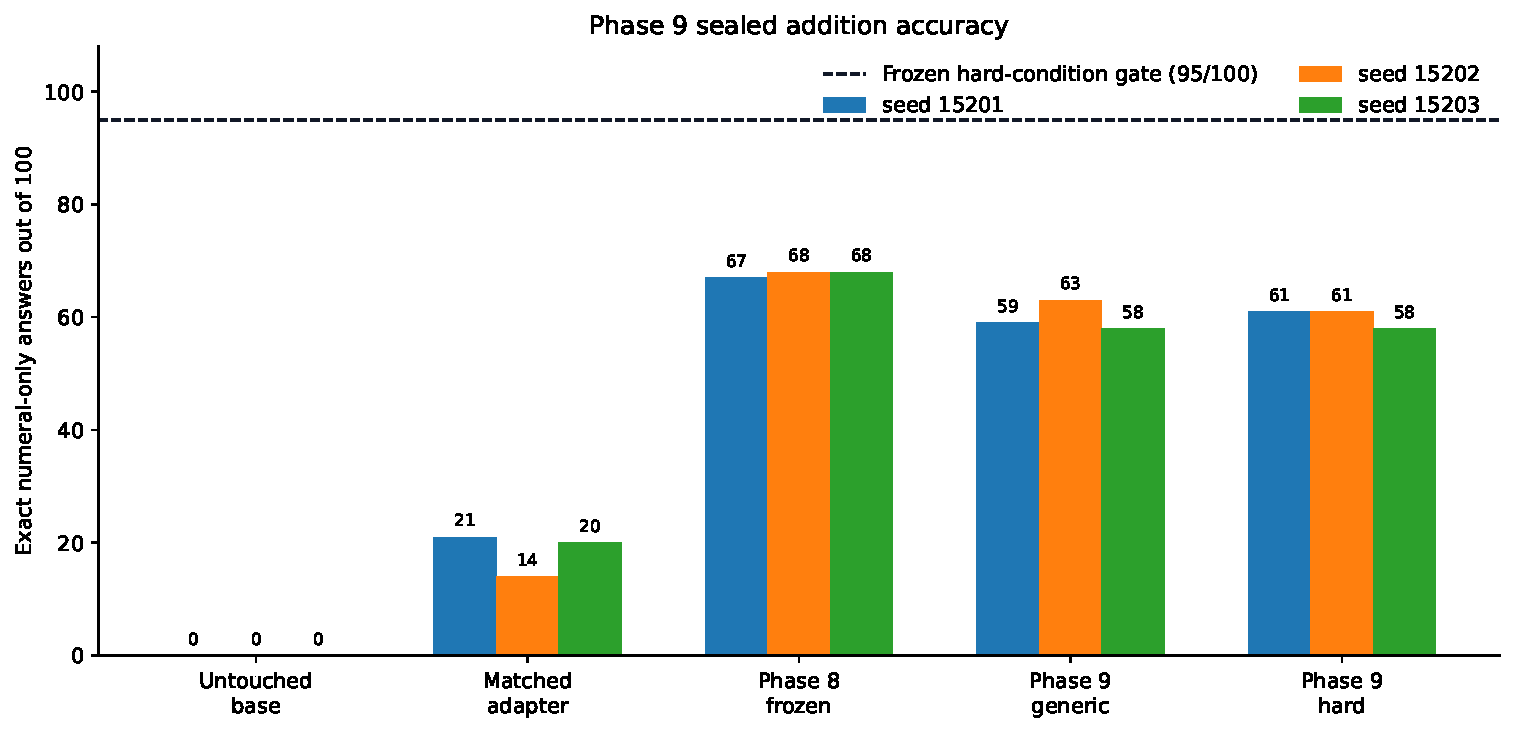
\includegraphics[width=\linewidth]{../phase9_figures/condition_accuracy.pdf}
\caption{Strict exact accuracy on the 100 sealed additions. The dashed line is
the frozen per-seed hard-condition gate. Hard continuation did not exceed
generic continuation in every seed and underperformed the unchanged Phase 8
implant.}
\end{figure}

The paired prompt changes were not a simple subset. Relative to Phase 8, hard
continuation gained 21, 19, and 17 newly correct prompts but lost 27, 26, and
27 previously correct prompts, for net changes of $-6$, $-7$, and $-10$.
Two-sided exact sign-test values were 0.471, 0.371, and 0.174; these are
descriptive rather than population-level inferential claims. Relative to
generic continuation, hard continuation changed exactness by $+2$, $-2$, and
0 prompts.

\subsection{Frozen gates}

\begin{center}
\small
\begin{tabular}{p{0.45\linewidth}p{0.28\linewidth}c}
\toprule
Gate & Observed hard result & Verdict\\
\midrule
Accuracy $\geq95/100$ per seed & 61, 61, 58 & \fail\\
Exact operands $\geq97/100$ & 85, 84, 81 & \fail\\
False routes $\leq4/200$ and preservation $\geq196/200$
  & 12/188, 12/188, 11/189 & \fail\\
All conditional trajectories and decodes exact
  & 61/61, 60/60, 57/57 & \pass\\
Paired causal losses $\geq90$ and ablated exact $\leq5$
  & 61/0, 61/0, 58/0 & \fail\\
Hard exact $>$ generic and hard false routes $\leq$ generic
  & $+2/-2/0$ exact; $+4/+4/+3$ false routes & \fail\\
\bottomrule
\end{tabular}
\end{center}

The compound protocol therefore failed.

\subsection{Disclosed conditional-gate implementation bug}

The frozen evaluator's raw gate Boolean reports the conditional mechanism as
false. Its implementation compares the total number of exact trajectories
among all positives with the number of active-route, exact-string-operand
examples. Seed 15,201 had equal counts, 61 and 61. Seeds 15,202 and 15,203
each had one additional exact trajectory from the register
\code{047 + 150}. That register is numerically equivalent and produced the
correct 197, but it does not exactly equal the target register
\code{47 + 150}. Total exact trajectories were therefore 61 and 58 while
protocol-defined conditional counts were 60 and 57, making the equality false.

Direct row-level recomputation evaluates the criterion as written: among
active-route examples whose operand registers exactly match the target, were
the calculator trajectory and decoded answer both exact? The answer is yes for
61/61, 60/60, and 57/57. The report therefore retains the raw implementation
flag and separately records the protocol-defined gate as a pass. This
correction does not change the compound failure because the other five gates
fail independently.

\section{Failure localization and causal evidence}

\subsection{Positive semantic trade-off}

Hard continuation substantially changed what the interface could recognize:

\begin{center}
\small
\begin{tabular}{lrrr}
\toprule
Hard positive category & Seed 15,201 & Seed 15,202 & Seed 15,203\\
\midrule
Direct exact / route / exact operands
  & 21 / 31 / 40 & 22 / 31 / 41 & 21 / 31 / 40\\
Word exact / route / exact operands
  & 20 / 20 / 25 & 20 / 20 / 25 & 20 / 20 / 25\\
Distractor exact / route / exact operands
  & 20 / 25 / 20 & 19 / 25 / 18 & 17 / 25 / 16\\
\bottomrule
\end{tabular}
\end{center}

The frozen Phase 8 interface answered 0/25 distractor additions in every seed;
hard continuation recovered 17--20/25. Exact operand registers increased from
73--74/100 in Phase 8 to 81--85/100. These are genuine gains in irrelevant
number rejection and state typing.

They did not compose with broad route recall. Exactly 24/100 positives were
routed off in each hard seed. Twenty belonged to four entire confirmation
families---three direct phrasings and one word-problem phrasing---and four
belonged to a fifth direct family. In many of these route-off prompts, the
separate operand rows still recovered both operands exactly. The router,
operand classifier, and active typed handshake therefore did not form one
globally coherent decision boundary.

Among the remaining failures, 10--11 had active routes but wrong operand
content, and 4--7 predicted addition but failed to activate the typed
handshake. No protocol-defined valid execution failed in the calculator or
downstream decoder.

\begin{figure}[ht]
\centering
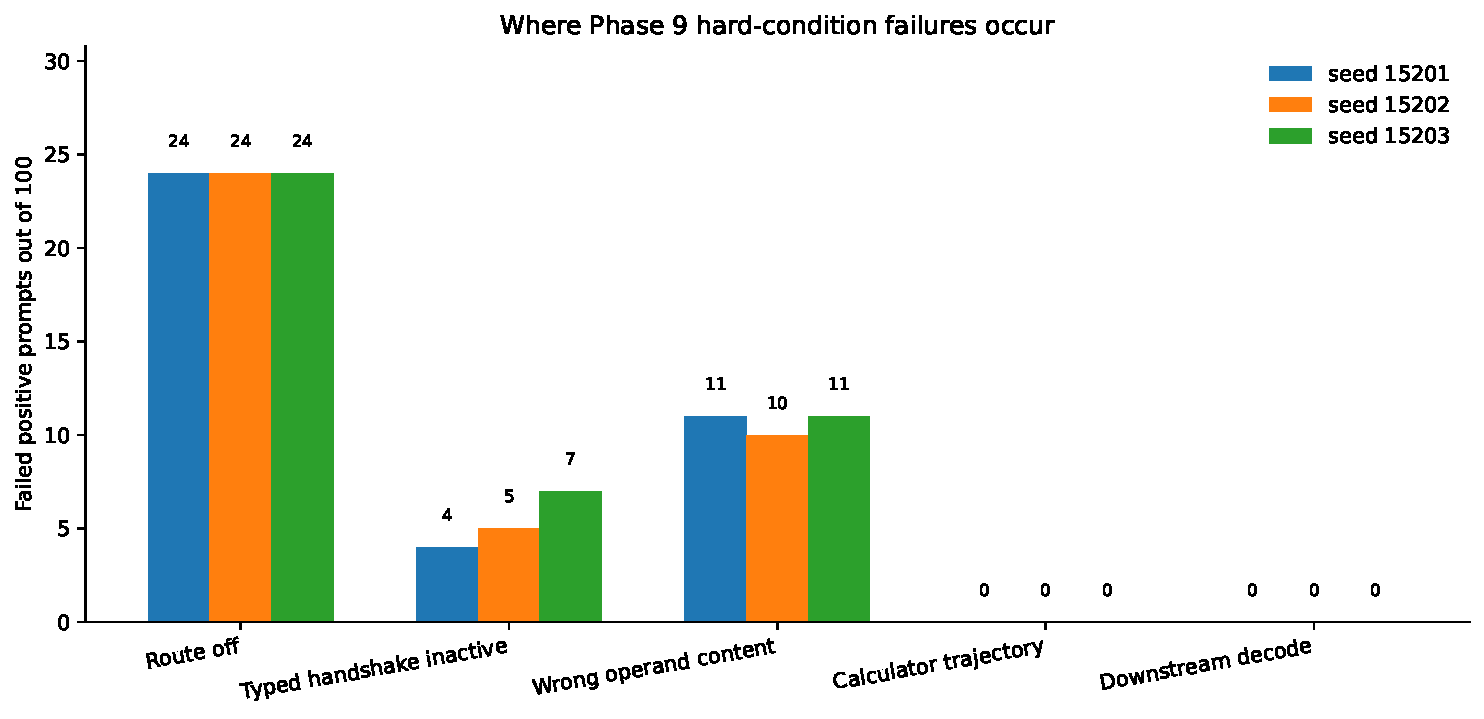
\includegraphics[width=0.94\linewidth]{../phase9_figures/hard_failure_taxonomy.pdf}
\caption{Mutually ordered failure stages for hard continuation. Route-off
errors dominate. No failure occurs after an exact typed interface reaches the
calculator.}
\end{figure}

Failure identity was highly correlated across seeds: 38 positive prompts
failed in all three seeds, while only 42 unique positive prompts failed in any
seed. This consistency argues against unlucky initialization as the primary
explanation.

\subsection{Adversarial routing}

Hard continuation reduced Phase 8 false routes from 30, 26, and 27 out of 200
to 12, 12, and 11. Token-exact preservation improved from 176, 178, and 178 to
188, 188, and 189. Paired preservation improved by 12, 10, and 11 prompts;
two-sided exact sign-test values were 0.00183, 0.00635, and 0.00098.

The frozen gate nevertheless required at most four false routes and at least
196 exact preservations. Generic continuation did better, with 8/200 route
predictions and 196/200 exact preservation in every seed. Its four additional
route predictions on three-number negatives did not activate the typed path
and therefore preserved base tokens.

Hard false routes were systematic:

\begin{center}
\small
\begin{tabular}{lrrr}
\toprule
Negative family & Seed 15,201 & Seed 15,202 & Seed 15,203\\
\midrule
Multiplication & 7/20 & 7/20 & 7/20\\
Canceled addition & 4/20 & 4/20 & 3/20\\
Concatenation & 1/20 & 1/20 & 1/20\\
Other seven families combined & 0/140 & 0/140 & 0/140\\
\bottomrule
\end{tabular}
\end{center}

\begin{figure}[ht]
\centering
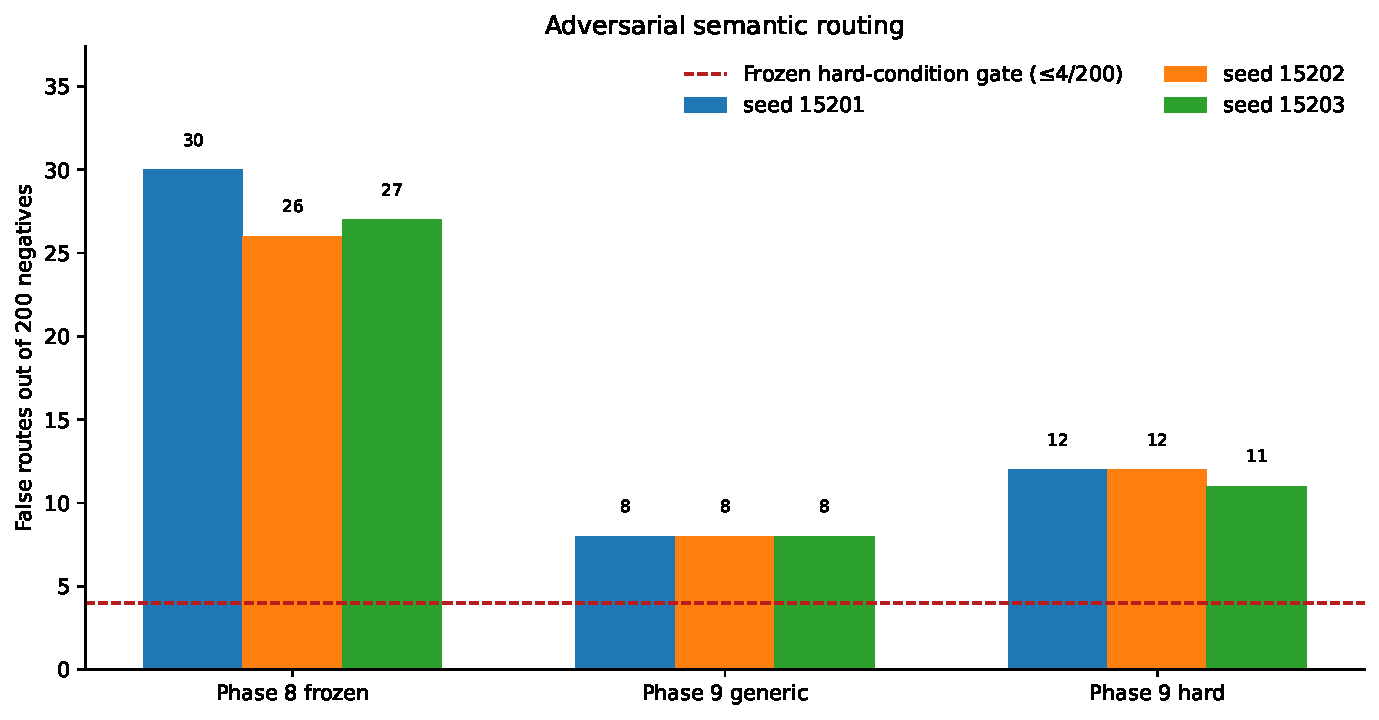
\includegraphics[width=0.92\linewidth]{../phase9_figures/negative_false_routes.pdf}
\caption{False route predictions on 200 adversarial negatives. Hard
continuation improves strongly over frozen Phase 8 but is worse than generic
continuation and misses the frozen gate.}
\end{figure}

\begin{figure}[ht]
\centering
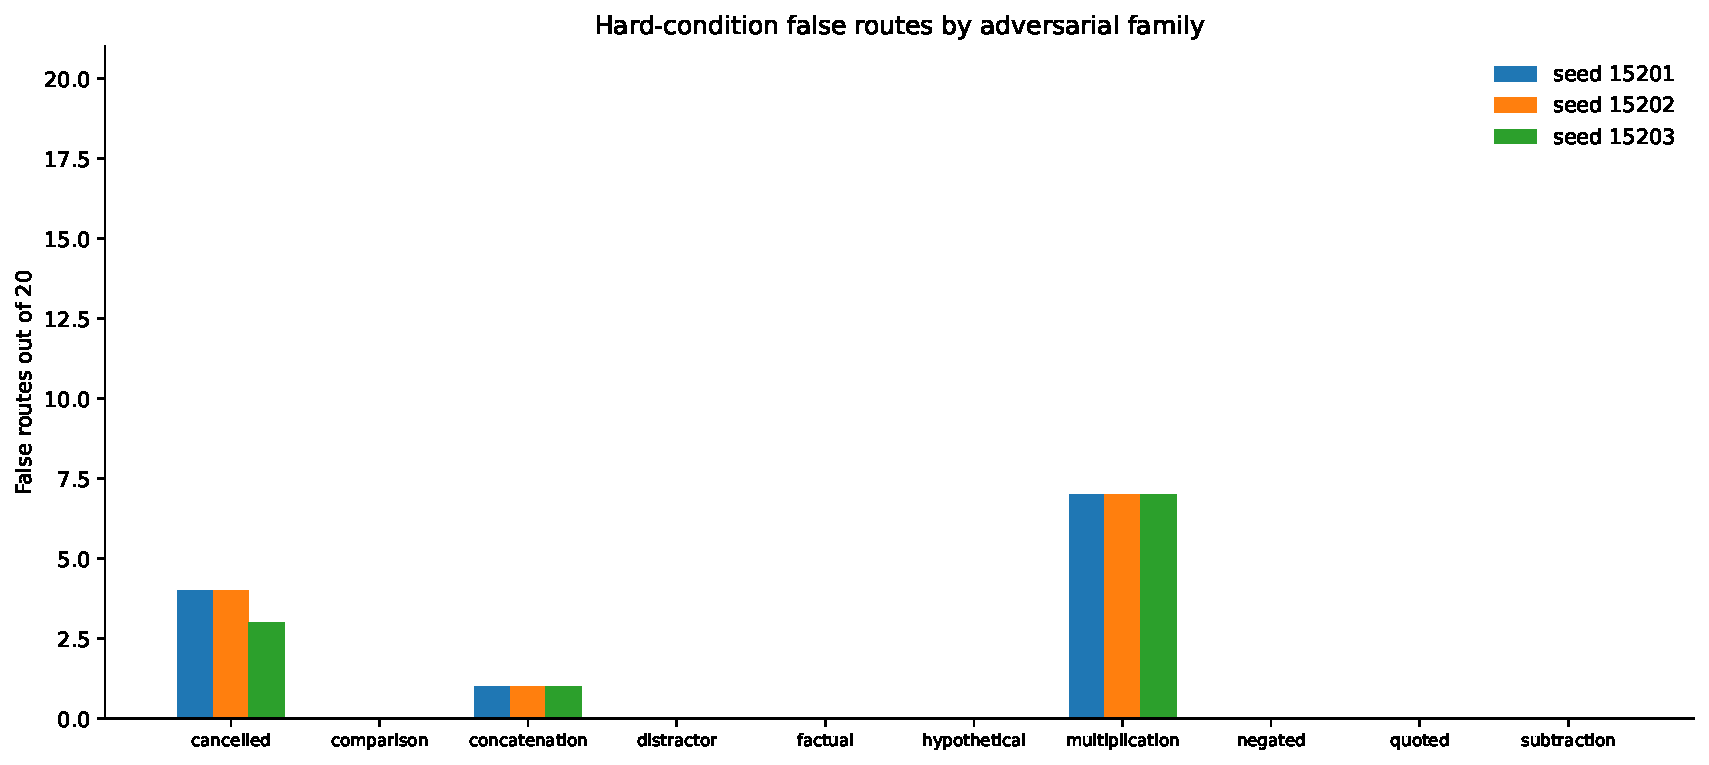
\includegraphics[width=\linewidth]{../phase9_figures/hard_false_routes_by_family.pdf}
\caption{Hard-condition false routes by adversarial family. The same
multiplication, cancellation, and concatenation failures recur across seeds.}
\end{figure}

\subsection{Deterministic execution and ablation}

Every active-route, exact-operand hard example followed the correct decimal
digit-plus-end trajectory and decoded to the exact numeral. Result-channel
ablation reduced all three seeds to 0/100. It caused 61, 61, and 58 paired
correct-to-incorrect changes---every available correct hard answer.

The causal gate still fails its fixed threshold of 90 paired losses because
end-to-end interface accuracy supplied only 58--61 correct cases to remove.
This is a threshold failure, not an observed failure of result-coordinate
dependence. The intervention evidence continues to localize the bottleneck
upstream of deterministic execution.

\section{Efficiency}

The implant architecture contains 57,344 learned weights, 0.005213\% of
TinyLlama's 1,100,048,384 parameters. Phase 9 updates only the 32,768 input
weights, 0.002979\% of the base. The deterministic calculator contains zero
learned parameters. The matched residual adapter contains exactly 57,344
learned weights but reaches only 14--21/100 additions and preserves 13--44/200
negative continuations token-for-token.

Median per-prompt latency was 1.135 seconds for untouched base. Hard
continuation medians were 1.019, 1.039, and 1.018 seconds; ablation medians
were 1.082, 1.069, and 1.086 seconds. Phase 8 implant medians were
0.963--0.977 seconds and generic continuation medians were
0.965--1.088 seconds. These are local implementation measurements, not claims
of hardware-independent speedup. Every generation deliberately recomputed the
full sequence without a KV cache.

The maximum sampled allocated MPS memory was 4,400,558,080 bytes (4.40 GB).
This samples current framework allocation after generations and is not a
device-driver peak watermark.

\section{Discussion}

\subsection{What Phase 9 establishes}

Phase 9 rejects the hypothesis that a count-matched hard semantic curriculum
is sufficient to make this frozen TinyLlama linear interface reliable. It also
rejects the simpler hypothesis that more generic continuation alone repairs
Phase 8. Both curricula average 60\% exact accuracy, below the unchanged
Phase 8 implant.

The negative result is more specific than ``TinyLlama cannot understand
arithmetic.'' Its frozen layer-15 states support several useful linear
readouts: hard training recovers more exact operands, learns most
three-number additions, and rejects many old adversarial families. But the
same 16 input rows do not maintain those gains while preserving broad
addition-intent recall and operation specificity. Family-level errors and
their cross-seed consistency indicate semantic distribution shift and limited
linear separability, not noisy arithmetic execution.

This supports, but does not uniquely prove, the earlier concern that the
TinyLlama base is a weaker representational substrate for this intervention.
Alternative explanations remain: layer 15 may be suboptimal for the expanded
families; the first-step linear route readout may be too restrictive; the
shared input rows and hard threshold may create an avoidable coordination
problem; or limited surrounding adaptation may be necessary. Phase 9 holds
those factors fixed and therefore cannot distinguish them.

\subsection{Why the deterministic-neuron hypothesis remains live}

The study does not show that integrating deterministic computation into neural
activations is ineffective. Conditional calculator execution remains perfect,
the frozen downstream model decodes every protocol-defined valid result, and
targeted result ablation removes every correct answer. The architectural
mechanism is causally operative.

What fails is the neural interface's ability to decide when to invoke that
mechanism and to create a fully valid typed state across arbitrary held-out
language. A perfect arithmetic cell cannot compensate for incorrect semantic
routing. This distinction is central to semi-deterministic AI: exact
subroutines require interfaces whose reliability is measured separately from
the programs they invoke.

\subsection{Next experiment}

The next phase should test interface capacity and representation while keeping
the calculator, output decoder, prompts, causal intervention, and preservation
logic fixed. A useful factorial design would compare:

\begin{enumerate}
\item the present linear route/role/digit readout;
\item a small nonlinear input interface with an exact learned-parameter match;
\item limited low-rank adaptation of the immediately surrounding TinyLlama
      representation;
\item an oracle-route diagnostic that isolates operand typing from semantic
      intent.
\end{enumerate}

Development selection should include explicit family-level positive-recall
constraints, not only aggregate recall under a false-positive cap. A new
exact-string-disjoint audit must be frozen before evaluating any repair. If a
small nonlinear interface succeeds while the linear one fails, the result
would identify interface capacity. If limited surrounding adaptation is
required, the bottleneck is representation accessibility. If neither works,
the model or layer becomes the leading explanation and a stronger
Llama-class replication is warranted.

Repeated invocation, multiple operations, and residual-native persistent state
should remain downstream goals until this interface problem is solved.

\subsection{Limitations and interpretation boundaries}

The base model, layer, activation bandwidth, and linear interface are held
fixed. Three interface seeds share one pretrained TinyLlama and one prompt
set. The study tests only four-digit decimal addition and short greedy
responses. It does not establish arbitrary-language robustness, spontaneous
calculator discovery, unlimited repeated invocation, general mathematical
reasoning, or semi-deterministic AI as a completed system.

Latency uses no KV cache. Sampled MPS allocated memory is not a driver-level
peak watermark. Paired prompt sign tests are descriptive because prompts and
seeds do not justify treating every row as an independent population sample.

\section{Reproducibility}

The frozen protocol is
\path{PHASE9_INTERFACE_HARDENING_PROTOCOL.md}. The exact prompt manifest is
\path{phase9_results/frozen_prompt_manifest.json}. Raw prompt-level outputs,
token traces, metrics, latency, memory samples, and checkpoint hashes are in
\path{phase9_results/confirmation.json}; the flat table is
\path{phase9_results/confirmation_rows.csv}; post-hoc decomposition and the
gate correction are in \path{phase9_results/analysis.json}. The chronological
record, including rejected development candidates and the infrastructure
retry, is \path{PHASE9_LAB_NOTEBOOK.md}.

SHA-256 values:

\begin{sloppypar}
\begin{itemize}
\scriptsize
\item frozen prompt manifest:
\code{70bb71fce29261eefd58f3ac2c4bb1caf2baff6aec8cdc3bf4bd69a9860aaf80};
\item confirmatory interface training:
\code{ea39989f5344d184c52e15adc86fb6f0702f31d91ae63f1a106b1f1600c60f01};
\item confirmation JSON:
\code{4b0f7ac5967fd6c3cd8a7c7f6ed6daf7e8c99c9132ff116035338136b76d1648};
\item confirmation CSV:
\code{6e06e86143a8bfe8017d2d03b2ecf07499bd0933741c761a6bb8ef5e6f8c0392};
\item post-hoc analysis:
\code{2e9d50b3dcd8d727967cc903592bafcf4e13ae83d8a54cda3c17b15ebb5f9ff9}.
\end{itemize}
\end{sloppypar}

Experiments ran on macOS 26.5.2 arm64 with Python 3.12.12, PyTorch 2.13.0,
Transformers 4.57.6, and Apple MPS. Large checkpoints remain in ignored local
artifact directories; their hashes and tensor invariants are retained in
tracked training, evaluation, and completion-audit records.

\section{Conclusion}

Phase 9 failed its frozen compound protocol. Hard semantic contrasts improved
operand recovery and several adversarial families, but they did not improve
overall addition accuracy, did not meet preservation requirements, and were
worse than generic continuation on negative routing. The interface learned
new families by losing old ones.

The result sharpens the architecture's boundary. The zero-parameter
deterministic calculator is exact when supplied a valid typed state, its result
is used by TinyLlama's native downstream computation, and its causal removal
eliminates every correct hard answer. Reliability is lost before execution:
at intent routing, route activation, and operand representation.

This is a meaningful negative result for semi-deterministic AI. Installing
exact neuron-shaped computation is feasible, but a small frozen linear
interface is not enough to make a weak language model invoke it robustly
across semantic distribution shift. The next scientific question is therefore
not whether to add more calculator operations. It is whether modest nonlinear
interface capacity or limited representation adaptation can solve the
routing-and-typing problem without sacrificing preservation.

\section*{Acknowledgment}

The deterministic-neuron hypothesis and semi-deterministic-AI research
direction were proposed by Josiah Wilson. Experimental design, implementation,
local execution, analysis, and drafting were conducted collaboratively with
OpenAI Codex under his direction. All frozen gates and observed failures are
retained.

\begin{thebibliography}{5}

\bibitem{trask2018}
A. Trask, F. Hill, S. Reed, J. Rae, C. Dyer, and P. Blunsom.
\newblock Neural Arithmetic Logic Units.
\newblock \emph{NeurIPS}, 2018.
\newblock \url{https://arxiv.org/abs/1808.00508}.

\bibitem{lindner2023}
D. Lindner, J. Kram\'{a}r, S. Farquhar, M. Rahtz, T. McGrath, and V. Mikulik.
\newblock Tracr: Compiled Transformers as a Laboratory for Interpretability.
\newblock \emph{NeurIPS}, 2023.
\newblock \url{https://arxiv.org/abs/2301.05062}.

\bibitem{bounsi2024}
W. Bounsi, B. Ibarz, A. Dudzik, J. Hamrick, L. Markeeva, A. Vitvitskyi,
R. Pascanu, and P. Veli\v{c}kovi\'{c}.
\newblock Transformers Meet Neural Algorithmic Reasoners.
\newblock 2024.
\newblock \url{https://arxiv.org/abs/2406.09308}.

\bibitem{tinyllama2024}
P. Zhang, G. Zeng, T. Wang, and W. Lu.
\newblock TinyLlama: An Open-Source Small Language Model.
\newblock 2024.
\newblock \url{https://arxiv.org/abs/2401.02385}.

\bibitem{dietz2025}
F. Dietz and D. Klakow.
\newblock IGC: Integrating a Gated Calculator into an LLM to Solve Arithmetic
Tasks Reliably and Efficiently.
\newblock 2025.
\newblock \url{https://arxiv.org/abs/2501.00684}.

\end{thebibliography}

\end{document}
